
\chapter{Phylogenetic Clustering (Phyloclustering)}
\label{chp:phyloclustering}


{\it
``What one man can invent another can discover.''\\
\--- Sherlock Holmes
}


\section{Introduction}

Phylogenetic Clustering (Phyloclustering)\index{phyloclustering}
discovers population structure based on information of DNA/RNA sequences
by combining two inventions: model-based clustering with evolutionary
models~\citep{Chen2011a}.
Note that what speaking here, regarding to ``evolutionary'',
is a mathematical/statistical model to interpret biological targets.
Neither religion nor theology is involved. 

In an over simplified case, suppose a sequence is composed by four nucleotides
$\mS = \{\colorA, \colorG, \colorC, \colorT\}$.
Assume a sequence
$\bx_n = \{x_{n1}, x_{n2},\ldots, x_{nL}\} \in \mS$
has $L$ loci (positions ordered) and is observed from a population, but
may have $K$ subpopulations that similar sequence patterns are expected
within each common subpopulation.
Each subpopulation is represented by a common center sequence
$\bmu_k = \{\mu_{k1}, \mu_{k2},\ldots, \mu_{kL}\} \in \mS$
which may or may not hypothetically exit in population and has to be
determined.
Therefore, each sequence has a probability mutated/evolved from any
center sequence. The higher the probability, the closer to the center
sequence.

The evolutionary model is based on a continuous time Markov chain
(CTMC)\index{continuous time Markov chain}\index{CTMC} on a state space $\mS$.
where the mutation process is characterized by
an instantaneously rate matrix $\bQ$ with dimension $4\times 4$,
i.e. rate at scale of tiny mutation time $t\rightarrow 0$.
We use the following steps to construct the likelihood function
as introduced in Chapter~\ref{chp:likelihood}:
\begin{enumerate}
\item
Given the above setting,
the mutation chance from a nucleotide $x$ to a nucleotide $y$ in time $t$ is
\begin{equation}
\Prob_{x, y}(t) = e^{\bQ_{x, y}t}
\label{eqn:e_Qt}
\end{equation}
for all $x, y \in \mS$.

\item
Assume each locus is mutated independently, then the mutation chance
(the transition probability) from $\bmu_k$ to $\bx_n$ in time $t$ is
$$
p_{\bmu_k, \bx_n}(t) = \prod_{l = 1}^L \Prob_{\mu_{kl}, \bx_{nl}}(t)
$$
for all $\bmu_{kl}, \bx_{nl} \in \mS$.

\item
Suppose there are $K$ subpopulations with mixing proportion $\eta_k$'s, then
the mutation chance from a sequence $\bmu_k$ to a sequence $\bx_n$ is
\begin{equation}
f(\bx_n; \btheta_K) = \sum_{k = 1}^K \eta_k p_{\bmu_k, \bx_n}(t)
\label{eqn:phyclust_mixture}
\end{equation}
where $\btheta_K = \{\eta_1, \eta_2, \ldots, \eta_{K-1},
                     \bmu_1, \bmu_2, \ldots, \bmu_{K}, \bQ, t\}$
are unknown and to be determined.
For simplicity, assume $\bQ$ and $t$ are identical across $K$ subpopulations.
Denote the distribution $\mF(\btheta_K)$ of the density function
$f(\bx_n; \btheta_K)$ for $\bx_n$.

\item
Suppose observed $N$ sequences $\bx = \{\bx_1, \bx_2, \ldots, \bx_N\}$
(each has $L$ loci)
independently and identically selected from unknown $K$ subpopulations
with mixing proportion $\boldeta$ to be estimated,
then the likelihood is
$$
L(\btheta_K; \bx) = \prod_{n = 1}^N f(\bx_n; \btheta_K).
$$
See Section~\ref{sec:likelihood_introduction} for construction.

\item
In short, the log likelihood is
\begin{eqnarray}
\log L(\btheta_K; \bx)
  & = & \sum_{k = 1}^K \log f(\bx_n; \btheta_K) \nonumber \\
  & = & \sum_{k = 1}^K \log
        \left[
        \sum_{k = 1}^K \eta_k p_{\bmu_k, \bx_n}(t)
        \right] \nonumber \\
  & = & \sum_{k = 1}^K \log
        \left[
        \sum_{k = 1}^K \eta_k
        \left(
        \prod_{l = 1}^L \Prob_{\mu_{kl}, \bx_{nl}}(t)
        \right)
        \right] \nonumber \\
  & = & \sum_{k = 1}^K \log
        \left[
        \sum_{k = 1}^K \eta_k
        \left(
        \prod_{l = 1}^L e^{\bQ_{\mu_{kl}, \bx_{nl}}t}
        \right)
        \right].
\label{eqn:phyclust_mixture_logl}
\end{eqnarray}

\end{enumerate}

Equation~(\ref{eqn:phyclust_mixture}) has similar structure
as Equation~(\ref{eqn:gaussian_mixture}). Therefore, the
EM algorithm~\citep{Dempster1977}\index{Algorithm!EM}
can be applied to maximize Equation~(\ref{eqn:phyclust_mixture_logl})
as maximize Equation~(\ref{eqn:gaussian_mixture_logl}).
Except the parameter space $\bTheta_K$ of
Equation~~(\ref{eqn:phyclust_mixture_logl}) where $\btheta_K$ belongs to
is neither continuous nor discrete space since $\bx_n$ and $\bmu_k$ are
in a categorical space which yields a very different E- and M-steps.


\section{The \pkg{phyclust} Package}
\label{sec:phyclust}

The \pkg{phyclust}~\citep{Chen2011a}
is an \proglang{R} package fully implements
phyloclustering with different configurations, EM algorithms, and
incorporating several useful tools such as \pkg{ms}~\citep{Hudson2002}
for simulating phylogeny and \pkg{seq-gen}~\citep{Rambaut1997}
for simulating sequence with vary mutations based on phylogenies.
The \pkg{phyclust} also provides functions for re-sampling sequences from
predicted models for determining an appropriate number of subpopulations.
Those functions are particular useful for Sections~\ref{sec:bootstrap}
and~\ref{sec:task_pull}.

The \pkg{phyclust} package has several example datasets which initials by
several longitudinal animal studies on horses about Equine Infectious Anemia
Virus (EIAV)~\citep{Leroux2004}\index{EIAV}.
See~\citet{Baccam2003} for more about the studies, horses, and their stories.

The EIAV is a lentivirus that
infects equine and causes Equine Infectious Anemia (EIA), and it is similar
to Human Immunodeficiency Virus (HIV) infects human and causes Acquired
Immunodeficiency Syndrome (AIDS).
Figure~\ref{fig:retrovirus}~\citep{Weiss2006}
shows a phylogeny of several relative lentivirus
in the retrovirus family, it also shows the closeness of EIAV and HIV which
makes the possible to building an animal model based on EIAV and study similar
mechanism further in HIV.
\begin{figure}[h!tb]
\centering
 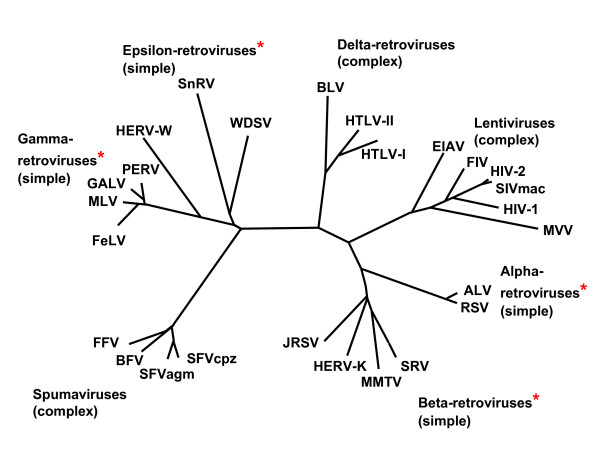
\includegraphics[width=5.0in]{pbdDEMO-include/pics/Phylogeny_of_Retroviruses}
\caption{Phylogeny of retroviruses originated from~\citet{Weiss2006}.}
\label{fig:retrovirus}
\end{figure}

The disease EIA progresses as the immune system
response to the viruses population change in blood which is collected
over time and generations. Part of blood samples are sequenced to identify
highly mutable coding regions with several overlapping reading frames. The
sequences and regions are then associated with disease progresses for
further analysis. Identify population structures is the critical step for
understanding the mutation patterns and designing better medicine or vaccine.

We perform phyloclustering on an example dataset,
{\it Pony 524}~\citep{Carpenter2011},\index{Data!Pony 524}
which is given in Figure~\ref{fig:eiav}.
It plots an example dataset where 146 EIAV sequences
are in y-axis and 405 loci in x-axis.
The top row is the consensus sequence, and only mutation sites are spotted
for 146 sequences. Colors represent \colorA, \colorC, \colorG, and
\colorT \ nucleotides. Three clusters fitted by a CTMC model are shown and
common mutation locations and types are grouped.
\begin{figure}[h!tb]
\centering
 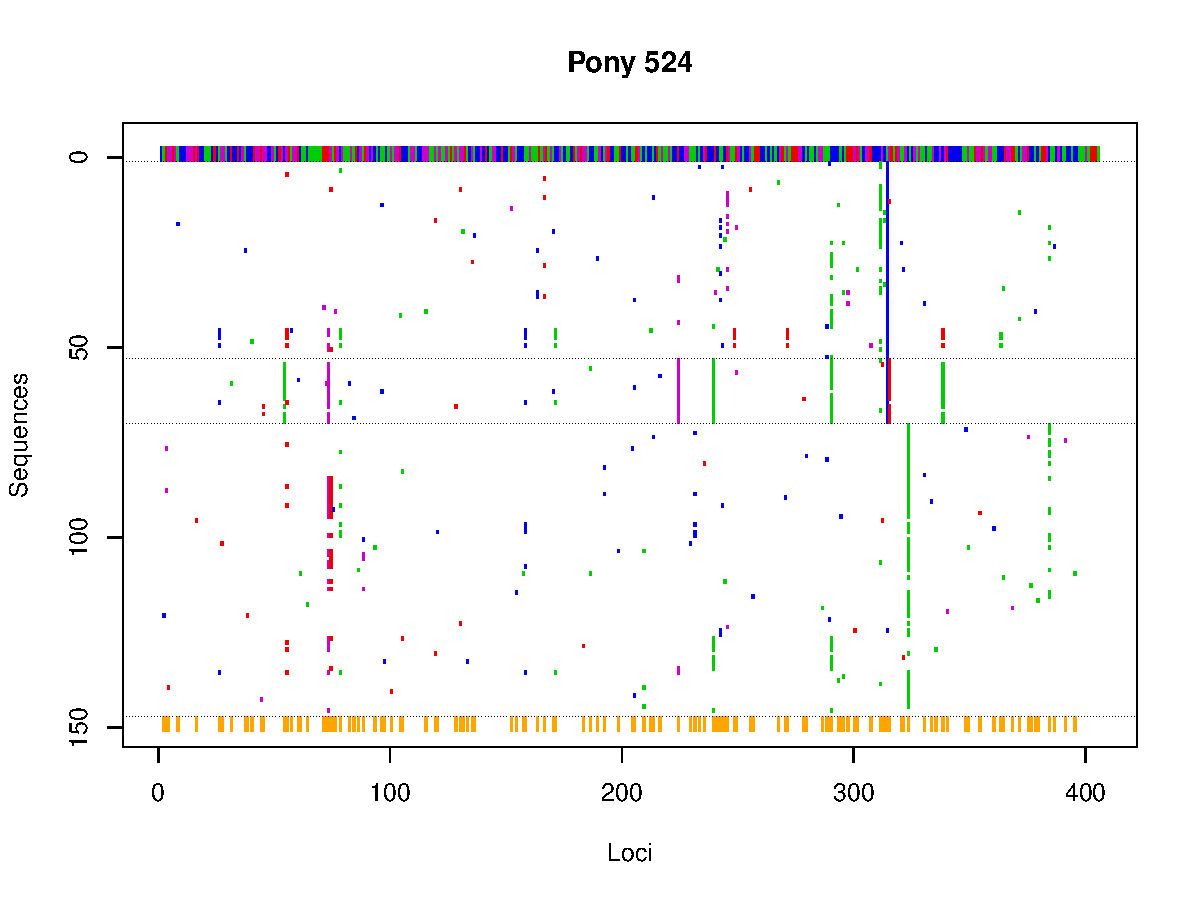
\includegraphics[width=6in]{pbdDEMO-include/pics/pony524}
\caption{146 EIAV sequences of {\it Pony 524}
in three clusters.}
\label{fig:eiav}
\end{figure}




\section{Bootstrap Method}
\label{sec:bootstrap}

``How many clusters are appropriate for the data?'' is a typical question
to any good scientists. There are several ways trying to infer this from
data in Statistics via hypothesis testing. For example,
$H_0: K = 2 \mbox{ v.s. } H_a: K = 3$ or more generally
$H_0: K = K^\prime \mbox{ v.s. } H_a: K = K^*$ for any $K^\prime \neq K^*$.
In mixture models, the nested parameter space is inappropriate, hence,
the LRT introduced in Section~\ref{sec:lrt} may not appropriate.

Bootstrap methods~\citep{Efron1979}\index{bootstrap}
may provide an adequate solution to
rebuild an asymptotic distribution for the likelihood ratio (LR).
``Asymptotic'' means ideally large sample size property.
The bootstrap methods is a re-sampling technique\index{re-sampling technique}
based on Monte Carlo\index{Monte Carlo} property
either from data (non-parametric)
or from model (parametric) to form a distribution for (LR).
Therefore, we may obtain a p-value by comparing LR to this distribution
rather than deriving an asymptotic distribution from LRT.

Phyloclustering which uses a mixture models with unusual parameter space
which is also particular suitable to apply the bootstrap methods to determine
an appropriate number of subpopulations.
For given data $\bX$ and hypothetical $K^\prime$ and $K^*$,
we may perform parametric bootstrap as the next.
\begin{enumerate}[label=Step \arabic*:]
\item
Based on $\bX$,
obtain MLEs $\hat{\btheta}_{K^\prime\,ML}$ and $\hat{\btheta}_{K^*\,ML}$
under $\bTheta_{K^\prime}$ and $\bTheta_{K^*}$, respectively.

\item
Compute and let
$
  \hat{\lambda} :=
  -2\log \hat{\Lambda}
  (\hat{\btheta}_{K^\prime\,ML},
   \hat{\btheta}_{K^*\,ML}; \bX).
$

\item
Sample new data $\bX^{(b)}$ from $\mF(\hat{\btheta}_{K^*\,ML})$.

\item
Based on $\bX^{(b)}$,
obtain MLEs $\hat{\btheta}^{(b)}_{K^\prime\,ML}$ and
$\hat{\btheta}^{(b)}_{K^*\,ML}$
under $\bTheta_{K^\prime}$ and $\bTheta_{K^*}$, respectively,
via the EM algorithm.

\item
Compute and let
$
  \lambda^{(b)} :=
  -2\log \hat{\Lambda}
  (\hat{\btheta}^{(b)}_{K^\prime\,ML},
   \hat{\btheta}^{(b)}_{K^*\,ML}; \bX^{(b)}).
$

\item
Repeat Steps 3 to 5 for $B$ times, collect and let
$\mF^{(B)}(\lambda) := \{\lambda^{(1)}, \lambda^{(2)}, \ldots, \lambda^{(B)}\}$
which is an approximation distribution to $\mF(\lambda)$,
the distribution of $\lambda$, as $B$ large enough.

\item
If $\hat{\lambda}$ greater than $q_{\mF^{(B)}(\lambda)}(0.95)$, then
we reject the $K^\prime$ model under $0.05$ level of type I error.

\end{enumerate}
Unlike LRT of Section~\ref{sec:lrt}, note that
$\hat{\btheta}_{K^*\,ML}$ is under $\bTheta_{K^*}$ rather than
$\bTheta_{K^\prime} \cup \bTheta_{K^*}$ nor $\bTheta_{K^\prime + K^*}$.
See \citet{Chen2011a} for more simulation studies of this approach via
\pkg{phyclust}.




\section{Task Pull Parallelism}
\label{sec:task_pull}

Obviously, Step 4 will be computationally intensive as $B$ increased,
and no guarantee that each of $b = 1,2,\ldots, B$ bootstrap sample
will take similar time at obtaining MLEs. It may be possible to parallelize
the EM algorithm fully in SPMD\index{Parallelism!SPMD} such as
Section~\ref{sec:parallel_model_based_clustering},
however, in general this step is still a bottleneck of whole computation.

The task parallelism\index{Parallelism!task parallelism}
as mention in Exercise~\ref{ch2:exercise:2}
is one way to solve the problem by simply divided jobs equally likely
to all processors.
This is probably an optimal solution for equal loading jobs
in homogeneous computing environment. However, it
will be a terrible solution for unbalance loading jobs or in-homogeneous
computing environment, such as
bootstrap methods introduced in Section~\ref{sec:bootstrap}.
Note that there are also some drawbacks for task parallelism:
\begin{itemize}
\item
it requires a processor to handle job controls as the role of manager in
manager/workers programming paradigm,\index{Parallelism!manager/works paradigm}
and
\item
the code is not obviously and difficult to debug or generalize.
\end{itemize}

The website
\href{http://math.acadiau.ca/ACMMaC/Rmpi/examples.html}{
http://math.acadiau.ca/ACMMaC/Rmpi/examples.html}
has a general view of task parallelism and examples in \pkg{Rmpi}.
Among three task parallel methods, task pull has the best performance and
suit for bootstrap methods.

A simplified example of task pull in SPMD can be found in the \pkg{pbdMPI}
demo via
\begin{lstlisting}
### At the shell prompt, run the demo with 4 processors by
### (Use Rscript.exe for windows system)
mpiexec -np 4 Rscript -e "demo(task_pull,'pbdMPI',ask=F,echo=F)"
\end{lstlisting}
which does the following
\begin{lstlisting}[language=rr,title=Task Pull Example]
### Initial
library(pbdDMPI, quiet = TRUE)

### Examples
FUN <- function(jid){
  Sys.sleep(1)
  jid * 10
}

ret <- task.pull(1:10, FUN)
comm.print(ret)

### Finish
finalize()
\end{lstlisting}
Note that lines 5 to 8 define a major function to be evaluated on all workers,
line 10 prepares 10 jobs from 1 to 10 where jobs can be done by any
available worker. The \code{task.pull()} is actually a combination of two
functions \code{task.pull.workers()} called by all workers and
\code{task.pull.master()} only called by the master by default rank 0.


\section{An Example Using the {\it Pony 524} Dataset}

As introduced in Section~\ref{sec:phyclust}, we will fit the 






\section{Exercises}
\label{sec:phyclust_exercise}

\begin{enumerate}[label=\thechapter-\arabic*]

\item
Argue that the instantaneously rate matrix $\bQ$ of Equation~\ref{eqn:e_Qt}
is positive definite. Therefore, argue that the
eigenvlaues decomposition\index{Decomposition!eigenvalues decomposition}
of $\bQ = \bU\bD\bU^{-1}$ exists. Prove that
$e^{\bQ t} = \bU e^{\bD t} \bU^{-1}$. Hence, this an easy way for
computing transition probability $\Prob_{x,y}(t)$.

\item
Argue that $\mF^{(B)}(\lambda)$ is a good approximation to $\mF(\lambda)$
in Step 4 of Section~\ref{sec:bootstrap}.

\end{enumerate}

